% --- watermark (auto-inserted) ---
% This manuscript is a grounded draft. The watermark block is preserved for the paper pipeline.
% --- end watermark ---
\documentclass[review,12pt]{elsarticle}

\usepackage{amssymb}
\usepackage{amsmath}
\usepackage{booktabs}
\usepackage{array}
\usepackage{float}
\usepackage{algorithm}
\usepackage{algorithmic}
\usepackage{hyperref}
\usepackage{lineno}

\begin{document}

\linenumbers
\begin{frontmatter}

\title{Pareto Memory Ranking Under Fixed Candidate Sets: Kernel Validation and Exploratory LongMemEval Session Reranking}

\author{Anonymous authors}

\begin{abstract}
Long-horizon agents often combine several memory objectives in a single scalar score, which can obscure trade-offs between freshness and relevance. This paper evaluates a bounded intervention: applying non-dominated sorting and crowding-distance selection after an existing candidate-generation step. The integrated long-term-memory adapter exposes similarity, retention, importance, and graph relevance, whereas the node-only timing path measures three objectives without graph state. A targeted Java run reports 14 tests with zero failures and zero errors, and a warmed $N=1000$, 1024-dimensional node-ranking microbenchmark reports a 2.537~ms median across nine measurements. We additionally run a frozen, offline LongMemEval-S raw-session reranking proxy: on 500 questions and 948 session labels, Pareto Recall@5 is 0.2529 versus 0.2559 for the fixed weighted-sum baseline, a descriptive difference of -0.003; 496 paired questions tie. The proxy uses BM25 lexical relevance, timestamp-derived retention, and missing importance set to zero, not Qwen embeddings or production summaries. JaCoCo reports 100\% class-level coverage for the Pareto ranker. These results support executable kernel contracts and an exploratory proxy comparison, not a significant retrieval gain, answer-quality improvement, or production end-to-end guarantee. The retrieval path also lacks a user identifier filter at the vector-query boundary, so tenant isolation and production safety are not established.
\end{abstract}
% @evidence[[paper_data.json#results]]
% @evidence[[results/kernel/memory-tests-final-14-post-coverage-fix.log#Tests run: 14, Failures: 0, Errors: 0]]
% @evidence[[results/kernel/memory-tests-final-14-post-coverage-fix.log#pareto_n1000_embedding1024_median_ms=2.537]]

\begin{graphicalabstract}
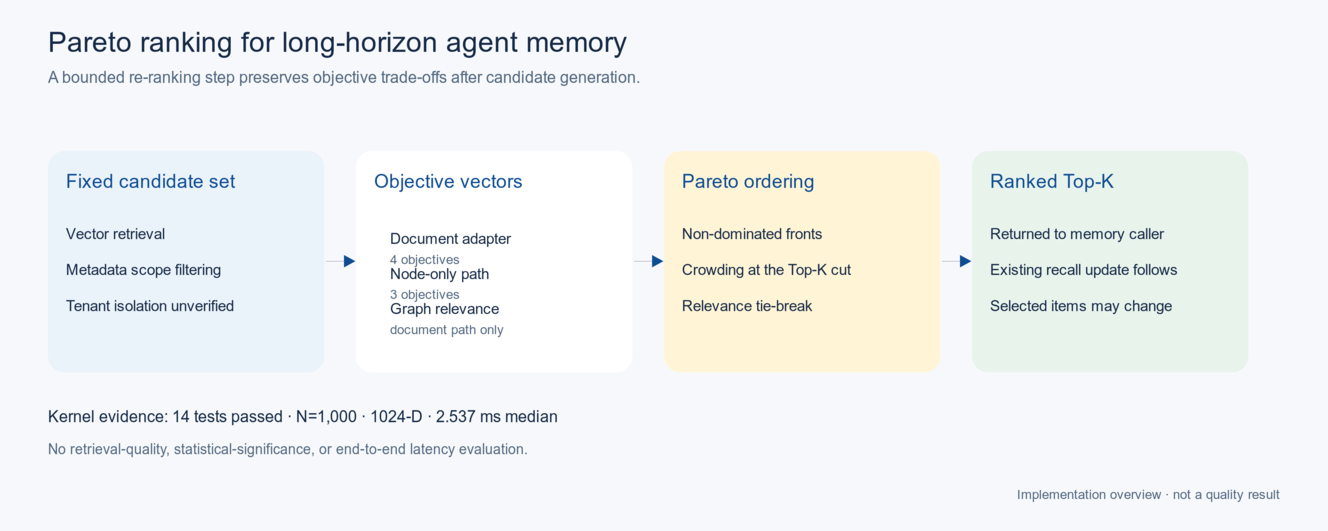
\includegraphics[width=\textwidth]{figures/graphical_abstract.png}
\end{graphicalabstract}
% @evidence[[figures/graphical_abstract.png.prov.json]]

\begin{highlights}
\item A minimal Pareto ranker is inserted after fixed-candidate retrieval.
\item Fourteen targeted tests pass in a run whose preamble reports OpenJDK 21.0.5.
\item A warmed kernel run takes 2.537 ms for 1,000 1,024-D candidates (median).
\item Pareto Recall@5 is 0.003 below weighted sum on LongMemEval.
\end{highlights}
% @evidence[[results/longmemeval_session_rerank/run_v2/summary.json#results.full]]

\begin{keyword}
long-term memory \sep multi-objective ranking \sep Pareto frontier \sep agent systems \sep reproducible microbenchmark
\end{keyword}

\end{frontmatter}

\section{Introduction}
\label{sec:introduction}

Long-horizon agents need to decide which stored memories should enter a bounded context. Long-term memory systems have explored retrieval, consolidation, and memory reinforcement as separate mechanisms; representative examples include MemoryBank~\cite{zhong2023memorybank} and long-context conversation memory~\cite{xu2022goldfish}. LongMemEval supplies question-level session evidence labels~\cite{wu2024longmemeval}, enabling a raw-session ranking proxy. Those labels do not map generated production summaries to source sessions, so the present experiment evaluates original sessions rather than the system's compressed-memory path.

The engineering question is therefore narrower: when the candidate set is already fixed, can a non-dominated ranker preserve objective trade-offs without changing candidate generation or the existing reinforcement rule? A weighted scalar score always imposes a single exchange rate between objectives. In contrast, non-dominated sorting keeps candidates that are incomparable across the objectives and uses crowding distance only when a front is larger than the requested output. The intervention is intentionally small: it changes ordering, not retrieval, storage, embedding, or answer generation.

This paper makes four bounded contributions. First, it describes the integration contract between the existing long-term memory path and a generic Pareto ranking kernel. Second, it records targeted tests that exercise strict dominance, incomparable trade-offs, crowding-distance boundary selection, invalid or empty inputs, graph-enabled integration, and no-graph fallback behavior. Third, it reports one warmed node-only microbenchmark on a fixed candidate set. Fourth, it provides a frozen offline LongMemEval-S raw-session comparison with an explicit weighted-sum baseline, while separating the proxy from production retrieval. The four-objective adapter and the three-objective node-only timing path are kept separate so that the timing result is not misread as a measurement of graph computation or production retrieval.

The central claim is correspondingly modest: the integrated kernel is functionally testable, has a millisecond-scale timing observation under the stated fixed-candidate protocol, and produces a small descriptive Pareto--weighted-sum difference under a raw-session lexical proxy. The paper makes no significance claim, no answer-quality claim, and no end-to-end production latency claim.

\section{Related Work}
\label{sec:related}

MemoryBank treats long-term memory as an explicit component for retaining information across interactions~\cite{zhong2023memorybank}. Beyond Goldfish Memory studies long-term open-domain conversation and motivates mechanisms that avoid treating every past message as equally useful~\cite{xu2022goldfish}. LongMemEval provides a benchmark framing for interactive memory, including session-level evidence labels across long histories~\cite{wu2024longmemeval}. Our use is limited to those raw-session labels and lexical proxy features; it does not reproduce the benchmark's full assistant-answer evaluation or establish quality for generated memory summaries.

The ranking mechanism uses standard multi-objective ideas: Pareto dominance separates candidates that are uniformly no worse from candidates that trade one objective against another, and crowding distance favors boundary and less-dense points within a front. These operations are related to the non-dominated sorting and crowding-distance mechanisms popularized by NSGA-II~\cite{deb2002nsga2}. Here they are used as a deterministic ranking primitive rather than as a population-based evolutionary optimizer. In particular, the cited optimization literature does not by itself imply a memory-retrieval gain for this system.

\section{Method}
\label{sec:method}

\subsection{Scope and interface}

Let $C=\{c_1,\ldots,c_n\}$ denote the candidate list returned by the existing memory path after its normal vector-store query and metadata scope filtering. The ranker receives $C$, a requested $k$, and objective vectors; it does not create new candidates, change embeddings, write to the vector store, or update reinforcement state. After ranking, the existing path continues with its retrieval-side reinforcement, so the selected objects may change even though the update mechanism itself is unchanged. This boundary makes the experiment a ranking-kernel study rather than an end-to-end retrieval study. Figure~\ref{fig:pareto-overview} summarizes the integrated path; it is an implementation overview, not an experimental result.
% @evidence[[paper_data.json#grounding_sources.retrieval-ranking-implementation]]
\begin{figure}[t]
\centering
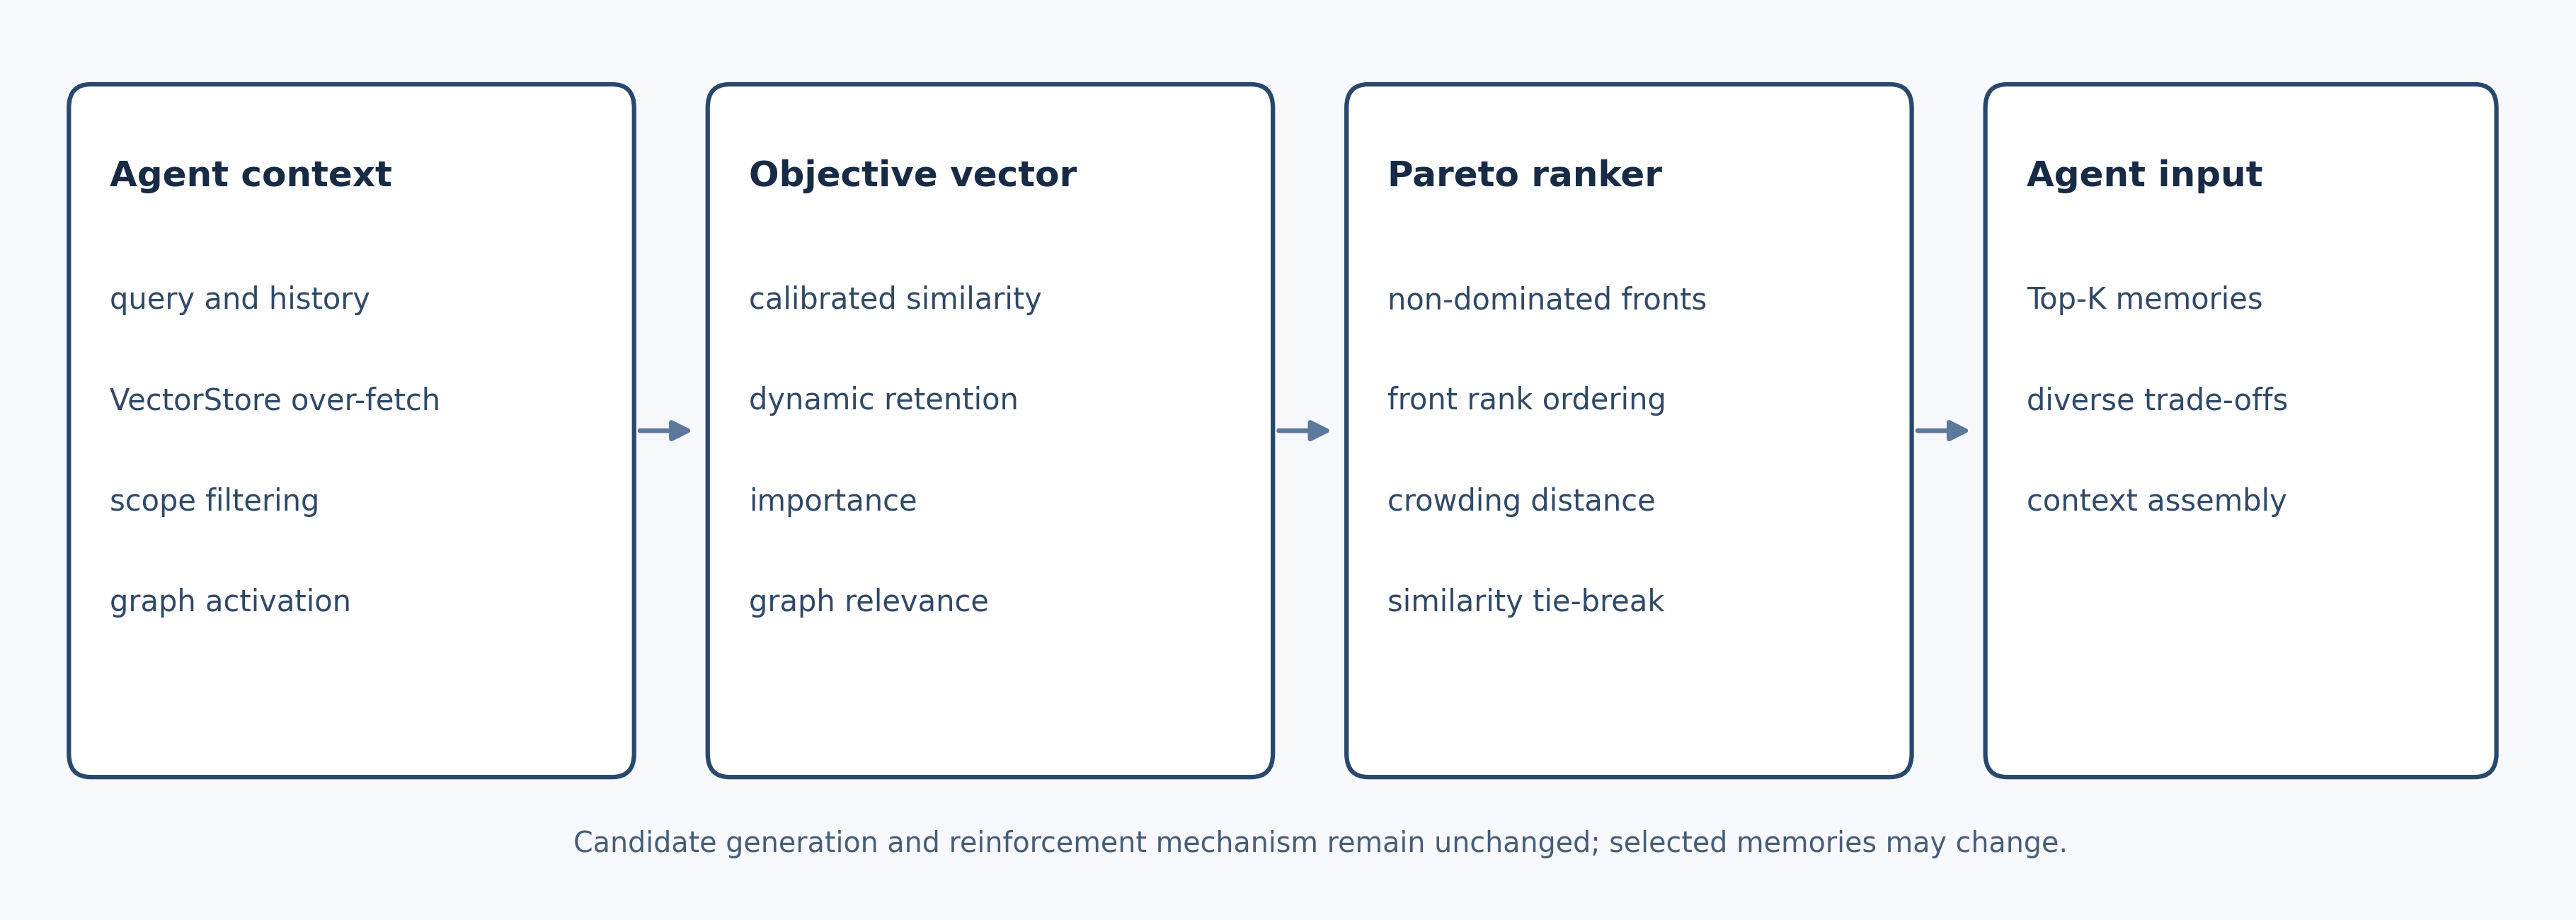
\includegraphics[width=\textwidth]{figures/pareto_memory_overview.png}
\caption{Conceptual implementation overview of the long-term memory ranking path. Candidate generation, scope filtering, and graph activation precede construction of the four-objective vector; Pareto ordering selects the Top-$K$ candidates. Downstream context assembly and agent task success are not evaluated in this study.}
\label{fig:pareto-overview}
\end{figure}

The long-term memory adapter constructs a four-dimensional objective vector
\begin{equation}
    f(c)=\bigl(s(c),\;r(c),\;i(c),\;g(c)\bigr),
    \qquad f_j(c)\in[0,1],
    \label{eq:four-objectives}
\end{equation}
where $s$ is calibrated similarity, $r$ is dynamic retention, $i$ is importance, and $g$ is graph relevance. The adapter therefore retains the existing objective computations and delegates only the ordering decision to the Pareto kernel. The node-only benchmark intentionally excludes graph state: it evaluates the three-dimensional vector $(r,s,i)$ available from a memory node, query embedding, and timestamp. Consequently, the reported latency is not a four-objective graph-path latency.
% @evidence[[paper_data.json#hypothesis]]

\subsection{Inherited dynamic-retention mechanism}

The ranker reuses the project's existing retention computations; it does not introduce a new forgetting law. In the document adapter, valid positive memory strength is reinforced after retrieval according to
\begin{equation*}
    S_{k+1}=\min\{3650,\max\{1,S_k[1+0.20\ln(1+k)]\}\},
\end{equation*}
where $k$ is the updated recall count and strength is measured in days. For retention scoring, importance is clipped to $\tilde I\in[0,1]$, then $S_{\mathrm{eff}}=S[1+0.5(\tilde I-0.5)]$ and $R=\exp(-\Delta d/S_{\mathrm{eff}})$, with age $\Delta d$ measured in days. The retrieved set is reinforced after ranking, so a changed order can change which memories receive that existing update.
% @evidence[[paper_data.json#grounding_sources.retrieval-ranking-implementation]]

The node-only scorer used in the timing test has a separate access-count-dependent decay implementation: $r(m,t)=\exp[-\lambda_0\Delta d/(1+0.50\ln(1+k))]$, with $k=\max(0,\mathrm{accessCount})$ and $\lambda_0$ taken from the node's positive decay rate or set to $0.05$. The two paths are reported separately because their score computations are not identical. Neither implementation uses semantic-association feedback to update strength; testing such a feedback-conditioned decay model is outside this study.
% @evidence[[paper_data.json#grounding_sources.retrieval-ranking-implementation]]

\subsection{Dominance and front construction}

For two candidates $a$ and $b$, $a$ dominates $b$ when
\begin{equation}
    f_j(a)\geq f_j(b)\quad\forall j,
    \qquad\text{and}\qquad
    f_{j^*}(a)>f_{j^*}(b)\quad\text{for at least one }j^*.
    \label{eq:dominance}
\end{equation}
Pairwise comparisons produce the first non-dominated front. Removing that front and repeating the comparison produces subsequent fronts. Front rank is therefore a partial-order signal: a candidate on a higher-priority front is not necessarily the best point on every individual objective, but it is not dominated by a candidate on a lower-priority front.

When a front contains more than $k$ candidates, the kernel computes normalized crowding distance independently along each objective, assigns infinite distance to objective boundaries, and selects the largest distances before using relevance as the deterministic tie-breaker. If the first front is smaller than $k$, complete fronts are appended in rank order and only the final partial front is truncated by crowding distance. This preserves extremes and avoids turning a trade-off into an arbitrary scalar exchange rate.

\subsection{Numerical and boundary semantics}

Objective values are normalized into the unit interval before comparison. Null or empty candidate lists and non-positive $k$ return an empty result. Objective vectors with inconsistent dimensions are rejected by the generic API; node-level vectors with an incompatible embedding length are skipped by the node adapter. These checks are part of the kernel contract, not additional benchmark assumptions.

The generic implementation uses pairwise dominance comparisons and per-objective sorting inside each selected front. With $n$ candidates and $d$ objectives, all-front construction has $O(n^2d)$ time and $O(n^2+nd)$ auxiliary space because pairwise dominance relations are retained; crowding-distance sorting adds at most $O(dn\log n)$ time. The three-objective node adapter's Fenwick-prefix first-front path runs in $O(n\log n)$ time and uses $O(n)$ auxiliary state, excluding the input nodes and embeddings. Including the per-node cosine calculation over embedding dimension $D$, its fast Top-$K$ path is $O(nD+n\log n)$ time. When the first front is smaller than $K$, it falls back to general front construction, giving $O(nD+n^2d)$ time and $O(n^2+nd)$ auxiliary space. The four-objective document adapter retains the generic path. The implementation keeps candidate objects and metadata intact; only the returned order changes.
% @evidence[[paper_data.json#grounding_sources.retrieval-ranking-implementation]]

\section{Experimental Protocol}
\label{sec:protocol}

The protocol freezes the candidate set at the call boundary and evaluates the kernel in a recorded Maven test run whose preamble prints OpenJDK 21.0.5; the archived output does not separately identify the JVM used by the Surefire fork. The targeted suite covers the ranker, dynamic-retention helper, and long-term-memory test classes (8, 3, and 3 tests, respectively). The ranker tests check dominance, trade-off fronts, crowding extremes, empty and invalid inputs, a fast-path parity case, fallback behavior, and the node-only timing path. The retention tests exercise the existing helper. The long-term-memory tests cover a two-document recall fixture, content-hash idempotency, and operation when graph activation is absent. The recall fixture requests $k=2$ for two candidates and checks only that both are returned, so it is a smoke test rather than evidence of adapter-level truncation or graph-driven ordering. These tests are diagnostic and contract-oriented; they are not a replacement for a benchmark with frozen retrieval labels.
% @evidence[[paper_data.json#grounding_sources.retrieval-ranking-implementation.locators.long_term_integration_tests]]

For the timing observation, the node-only ranker receives a fixed list of $N=1000$ candidates with 1024-dimensional normalized vectors and returns a bounded top-$k$ list. The JUnit measurement is warmed before the recorded samples and reports the median elapsed time. The result is reported as an observation on one machine and one runtime configuration, not as a production percentile or a hardware-independent guarantee.
% @evidence[[paper_data.json#results.n1000_embedding_dimensions]]
% @evidence[[paper_data.json#results.n1000_median_latency_ms]]
% @evidence[[results/kernel/memory-tests-final-14-post-coverage-fix.log#pareto_n1000_embedding1024_sorted_samples_ns]]

The external benchmark analysis is a separate raw-session proxy rather than a replay of the production path. We use the repository-local LongMemEval-S cleaned set, with 500 questions and 948 \texttt{answer\_session\_ids} labels. Query and session text are tokenized as lowercase ASCII alphanumeric terms, and BM25 uses $k_1=2$, $b=0.75$, and $\ln[(N-df+0.5)/(df+0.5)]$ IDF~\cite{perez2009bm25lucene}; negative raw scores are clipped to zero and mapped to $x/(1+x)$. Retention is $\exp[-0.05\max(0,\Delta d)/(1+0.5\ln(1+0))]$, where $\Delta d$ is the age in days at the question date. Importance is fixed at the missing-value default of zero. Thus only lexical relevance and retention vary. Pareto ranking uses non-dominated fronts and normalized crowding distance; the matched scalar baseline uses $0.25r+0.35i+0.40s$, where $i=0$ and $s$ is the bounded lexical proxy. Both methods receive the same candidate positions and features, use stable index tie-breaking, and are evaluated at $K=5$ and $K=10$. No answers enter feature construction or ranking. We evaluate all 500 questions descriptively and perform no significance test because shared candidate IDs connect the questions into a single component. The proxy does not use Qwen embeddings or generated production summaries.
% @evidence[[results/longmemeval_session_rerank/experiment_contract.json]]
% @evidence[[results/longmemeval_session_rerank/run_v2/summary.json.prov.json]]

The supplied candidate arrays contain 13 within-question repeated non-qrel session identifiers paired with distinct dates; their positions are preserved and ranked separately, while hit metrics count unique session IDs. In addition, 75 qrel labels are future-dated relative to their question date. The primary analysis retains the supplied full haystack; the strict date-cutoff sensitivity analysis retains all original qrels and counts unavailable labels as misses.
% @evidence[[results/longmemeval_session_rerank/run_v2/summary.json#dataset]]

\section{Results}
\label{sec:results}

\subsection{Contract-level correctness}

The recorded targeted run completed all 14 tests with zero failures and zero errors; the log preamble prints OpenJDK 21.0.5 but does not identify the Surefire fork JVM separately. The result confirms that the exercised contracts execute successfully in that recorded run. It does not establish that every production integration or every candidate distribution is covered.
% @evidence[[results/kernel/memory-tests-final-14-post-coverage-fix.log#Tests run: 14, Failures: 0, Errors: 0]]

\begin{table}[t]
\centering
\caption{Grounded evidence boundary for the reported study.}
\label{tab:evidence-boundary}
\begin{tabular}{p{0.28\linewidth}p{0.19\linewidth}p{0.39\linewidth}}
\toprule
Artifact or path & Observation & Interpretation \\
\midrule
Targeted test run & 14 tests; 0 failures; 0 errors & The log preamble prints OpenJDK 21.0.5; Surefire fork runtime is not separately recorded. \\
Node-only timing path & $N=1000$; 1024 dimensions; 2.537~ms median & Warmed microbenchmark observation for the three-objective node ranker. \\
Pareto-ranker coverage & 100\% each & Class-level JaCoCo counters; not project-wide coverage. \\
LongMemEval-S raw-session proxy & 500 questions; 948 qrels; BM25 features & Descriptive proxy only; not Qwen, compressed-memory, or answer-quality evaluation. \\
Pareto vs. weighted-sum Recall@5 & 0.2529 vs. 0.2559; delta -0.003 & 496 ties; one connected overlap component; no significance claim. \\
\bottomrule
\end{tabular}
\end{table}
% @evidence[[paper_data.json#results]]
% @evidence[[results/longmemeval_session_rerank/run_v2/summary.json#results.full]]
% @evidence[[results/kernel/memory-tests-final-14-post-coverage-fix.log]]
% @evidence[[results/kernel/pareto-jacoco-report-post-coverage-fix.csv#ParetoMemoryRanker]]

The ranker tests include strict-dominance and incomparable trade-off cases, and check that crowding-distance truncation retains objective-boundary candidates. Null, empty, and dimension-mismatch inputs exercise fail-safe behavior. In the adapter fixture, both candidates are returned because $k=2$; it does not assert ordering, exercise truncation, or verify that graph activation changes the result. The generic ranker tests exercise truncation separately. These observations support selected kernel contracts. On the corrected frozen raw-session proxy, Pareto macro Recall@5 is 0.2529 versus 0.2559 for the fixed weighted-sum baseline (paired descriptive difference -0.003); 1 question favors Pareto, 496 tie, and 3 favor the baseline. Micro Recall@5 is 0.2205 versus 0.2226, and macro nDCG@5 is 0.2122 versus 0.2137. The point differences are small and descriptive only. All questions belong to one shared-session component, so the 500 rows are not treated as independent evidence for a p-value or a generalization claim.
% @evidence[[results/kernel/memory-tests-final-14-post-coverage-fix.log#Tests run: 14, Failures: 0, Errors: 0]]
% @evidence[[paper_data.json#grounding_sources.retrieval-ranking-implementation.locators.long_term_integration_tests]]
% @evidence[[results/longmemeval_session_rerank/run_v2/summary.json#results.full]]

The class-level JaCoCo report records 100\% instruction, branch, line, and method coverage for \texttt{ParetoMemoryRanker}. These figures are class-level diagnostics and should not be summarized as 100\% overall or project-wide coverage.
% @evidence[[paper_data.json#results.pareto_ranker_coverage_percent]]
% @evidence[[results/kernel/pareto-jacoco-report-post-coverage-fix.csv#ParetoMemoryRanker]]

\subsection{Node-only microbenchmark}

The warmed node-only path reports a median latency of 2.537~ms for $N=1000$ and 1024-dimensional candidates. The measured path computes three objective values per node, performs non-dominated comparisons, and applies crowding distance when required. It does not include external vector-store latency, graph activation, embedding generation, network transfer, persistence, or model generation. The number is therefore useful as a kernel-scale reference point and not as an end-to-end service budget.
% @evidence[[results/kernel/memory-tests-final-14-post-coverage-fix.log#pareto_n1000_embedding1024_median_ms=2.537]]
% @evidence[[paper_data.json#results.n1000_median_latency_ms]]

\subsection{LongMemEval session-level proxy comparison}
\label{sec:longmemeval}

Table~\ref{tab:longmemeval} reports the full-haystack primary comparison. Pareto ranking is 0.003 lower in macro Recall@5 than the frozen weighted-sum baseline, a small descriptive difference rather than evidence of statistically reliable superiority. One question favors Pareto, 496 are tied, and three favor weighted sum. Because candidate sessions overlap across questions and the overlap graph is connected, we do not interpret question-level outcomes as independent replicates. Under the strict question-date cutoff, macro Recall@5 is 0.2494 for Pareto and 0.2524 for weighted sum; micro Recall@5 is 0.2152 and 0.2173, respectively, with 75 future-dated qrels retained as misses in both methods' denominators.
% @evidence[[results/longmemeval_session_rerank/run_v2/summary.json#results.full]]
% @evidence[[results/longmemeval_session_rerank/run_v2/summary.json#results.asof]]

\begin{table}[t]
\centering
\caption{Frozen LongMemEval-S raw-session reranking proxy. Scores are descriptive; the lexical feature is BM25 rather than production Qwen cosine relevance.}
\label{tab:longmemeval}
\begin{tabular}{lrrr}
\toprule
Metric & Pareto & Weighted sum & Difference \\
\midrule
Macro Recall@5 & 0.2529 & 0.2559 & -0.0030 \\
Micro Recall@5 & 0.2205 & 0.2226 & -0.0021 \\
Macro nDCG@5 & 0.2122 & 0.2137 & -0.0015 \\
Hit@5 & 0.3760 & 0.3780 & -0.0020 \\
Macro Recall@10 & 0.3764 & 0.3764 & 0.0000 \\
Micro Recall@10 & 0.3449 & 0.3449 & 0.0000 \\
\bottomrule
\end{tabular}
\end{table}
% @evidence[[results/longmemeval_session_rerank/run_v2/summary.json#results.full]]
% @evidence[[results/longmemeval_session_rerank/run_v2/summary.json.prov.json]]

\subsection{What the evidence does not show}

The LongMemEval comparison measures session-level retrieval under a lexical proxy on original raw sessions. It does not test the system's compressed-memory candidates, Qwen/cosine relevance, generated answers, answer faithfulness, or end-to-end task success. The observed -0.003 macro Recall@5 difference slightly favors the weighted baseline, with 496 questions tied, and cannot be promoted to a general or statistically significant claim under the connected overlap structure. The timing microbenchmark remains separate from this dataset-level ranking calculation.
% @evidence[[paper_data.json#limitations]]
% @evidence[[results/longmemeval_session_rerank/experiment_contract.json]]
% @evidence[[results/longmemeval_session_rerank/run_v2/summary.json#interpretation]]

\section{Limitations}
\label{sec:limitations}

The evidence is intentionally narrow. First, the timing path is a warmed JUnit microbenchmark on one machine, so it should not be read as a p50/p95 production measurement. Second, the timing path uses 1024-dimensional node vectors and excludes graph activation; it is not a measurement of the four-objective adapter under a production embedding or vector-store workload. Third, the LongMemEval comparison uses original raw sessions, a complete BM25 lexical proxy, timestamp-derived retention, and missing importance set to zero; it does not evaluate Qwen embeddings, generated summaries, answer quality, or end-to-end agent success. Fourth, the corrected macro Recall@5 point estimate is 0.003 lower for Pareto, with 496 of 500 paired observations tied, and the connected session-overlap structure prevents an independent-question significance or generalization claim. Fifth, 13 questions contain repeated non-qrel candidate IDs with distinct dates; retaining them by position follows the source alignment but is a data irregularity that may affect position-wise ranking. Sixth, 75 qrel labels are future-dated relative to their question date; the primary full-haystack analysis preserves them, while the strict-cutoff sensitivity treats them as unavailable misses. Seventh, JaCoCo reports 100\% branch coverage for the ranker, but this remains a class-level diagnostic and does not establish complete project-wide control-flow coverage. Eighth, the adapter trade-off fixture has two candidates and $k=2$ and checks membership only; it does not test adapter-level truncation, order, or graph-activation effects. The generic ranker tests cover truncation separately. The successful targeted log reports test classes as up to date rather than freshly compiled; a later full test-source compilation stopped on errors in unrelated Phase 151/152 benchmark tests before the targeted suite ran. Thus the archived pass is a successful recorded run but is not a fresh compile-and-test proof for the current source snapshot. Finally, the long-term-memory code path does not establish user-level isolation: the vector-store request supplies the query and top-$k$, after which scope filtering is applied; the user identifier is derived from returned candidates for graph activation rather than applied as a vector-query filter. If users share a scope, this path does not by itself exclude cross-user candidates. The current tests therefore do not establish tenant isolation, and this security boundary requires separate remediation and verification before production safety can be claimed. The correct interpretation is feasibility and exploratory proxy evidence, not production superiority or isolation assurance.
% @evidence[[paper_data.json#limitations]]
% @evidence[[paper_data.json#grounding_sources.retrieval-ranking-implementation.locators.long_term_integration_tests]]
% @evidence[[paper_data.json#grounding_sources.test-compilation-diagnostic-20261029]]

\section{Conclusion}
\label{sec:conclusion}

This study isolates one engineering change: Pareto-frontier ordering after a fixed candidate set. The existing long-term-memory adapter can express four objectives, while the node-only benchmark measures the three-objective ranker that is independent of graph state. The recorded targeted run passed 14 tests with no failures or errors; its log preamble prints OpenJDK 21.0.5 but does not identify the Surefire fork JVM separately. The warmed $N=1000$, 1024-dimensional kernel observation was 2.537~ms median. The class-level report gives 100\% instruction, branch, line, and method coverage. In the corrected frozen LongMemEval-S raw-session proxy, Pareto macro Recall@5 was 0.2529 versus 0.2559 for weighted sum, a descriptive -0.003 difference with 496 ties; strict cutoff sensitivity also favored the baseline by 0.003. These observations support exercised contracts and an exploratory proxy comparison, not significant retrieval or answer-quality gains, Qwen-vector performance, or end-to-end service performance. The retrieval path's user isolation also remains unverified because the vector query is not filtered by user identifier. A subsequent study would need an independently controlled production-candidate mapping, semantic embedding features, and separate remediation and verification of tenant isolation.
% @evidence[[paper_data.json#results]]
% @evidence[[paper_data.json#limitations]]

\section*{Funding}
Funding information was not supplied with the study artifacts and must be confirmed by the authors before submission.

\section*{Declaration of competing interest}
A competing-interest statement was not supplied with the study artifacts and must be confirmed by the authors before submission.

\section*{Data availability}
The manuscript uses repository-local kernel logs and the corrected frozen LongMemEval-S raw-session proxy artifacts described in the evidence table. The proxy input is retained under \texttt{data/external/longmemeval}; it is not a generated-summary or answer-quality evaluation.

\section*{Code availability}
The ranking kernel and its targeted tests are part of the accompanying project worktree. The manuscript does not modify the production source as part of the paper-writing step.

\section*{CRediT authorship contribution statement}
Author contributions were not supplied with the study artifacts and must be completed by the authors before submission.

\section*{Declaration of generative AI and AI-assisted technologies in the writing process}
During the preparation of this manuscript, an AI-assisted tool was used to help organize prose and check consistency against the repository-local evidence. This manuscript is a draft; the authors must review and edit the content as needed and take full responsibility before submission.

% IMPORTANT: flush all floats before the bibliography so that supplementary material is rendered after references.
\nolinenumbers
\clearpage
\bibliographystyle{elsarticle-num}
\bibliography{references}

\clearpage
\appendix
\section{Supplementary Information}
\label{sec:supplementary}

\subsection{Reproducibility record}
\label{sec:si-repro}

The reproducibility record consists of the project-local compilation log, targeted test log, JaCoCo report, and paper-data summary. The targeted log preamble prints the OpenJDK 21.0.5 version string and records three test classes, their individual counts, the aggregate count, and the node-only timing samples; it does not retain the invoking shell command, identify the Surefire fork JVM separately, and reports test compilation as up to date. A later diagnostic rerun attempted to compile the test sources but stopped on Phase 151/152 benchmark test errors before Surefire, so it produced no newer targeted result. The JaCoCo CSV is the class-level report used for the coverage statement. The successful targeted log and paper-data summary provide the quantitative values reported in this manuscript.
% @evidence[[results/kernel/core-compile-post-coverage-fix.log]]
% @evidence[[results/kernel/memory-tests-final-14-post-coverage-fix.log]]
% @evidence[[results/kernel/memory-tests-final-14-integration-fix.log]]
% @evidence[[results/kernel/pareto-jacoco-report-post-coverage-fix.csv]]
% @evidence[[paper_data.json]]

An independent execution of the frozen LongMemEval contract passed all ten built-in self-checks. Its dataset, results, and interpretation objects matched the accepted run; the full and strict-cutoff per-question CSV files were byte-identical. This confirms reproducibility of this offline proxy execution, not independent-sample inference or generalization beyond its connected question/session set.
% @evidence[[results/longmemeval_session_rerank/reproduction_check_20261029/summary.json.prov.json]]
% @evidence[[results/longmemeval_session_rerank/reproduction_check_20261029/per_question_metrics.csv.prov.json]]
% @evidence[[results/longmemeval_session_rerank/reproduction_check_20261029/per_question_asof_metrics.csv.prov.json]]

\begin{table}[H]
\centering
\caption{Targeted test inventory recorded in the final kernel log.}
\label{tab:si-tests}
\begin{tabular}{p{0.42\linewidth}c p{0.36\linewidth}}
\toprule
Test class & Tests & Main contract \\
\midrule
\texttt{LongTermMemoryEnhancedTest} & 3 & 2-candidate/$k=2$ recall smoke test, idempotency, and no-graph fallback \\
\texttt{ParetoMemoryRankerTest} & 8 & Dominance, trade-offs, crowding, boundaries, ties, fallback, and timing \\
\texttt{DynamicEbbinghausDecayTest} & 3 & Existing retention helper behavior \\
\midrule
Aggregate & 14 & 0 failures; 0 errors \\
\bottomrule
\end{tabular}
\end{table}
% @evidence[[results/kernel/memory-tests-final-14-post-coverage-fix.log#Tests run: 3, Failures: 0, Errors: 0]]
% @evidence[[results/kernel/memory-tests-final-14-post-coverage-fix.log#Tests run: 8, Failures: 0, Errors: 0]]
% @evidence[[results/kernel/memory-tests-final-14-post-coverage-fix.log#Tests run: 14, Failures: 0, Errors: 0]]

\subsection{Ranking pseudocode and invariants}
\label{sec:si-pseudocode}

The kernel can be summarized without reference to a dataset-specific score scale:
\begin{algorithm}[H]
\caption{Pareto ranking and Top-$K$ truncation}
\label{alg:pareto-topk}
\begin{algorithmic}[1]
\REQUIRE Candidate vectors $C$, output limit $K$
\ENSURE Ordered candidate list $L$ with $|L|\leq K$
\IF{$C=\emptyset$ or $K\leq 0$}
    \RETURN $[\ ]$
\ENDIF
\STATE Partition $C$ into non-dominated fronts $F_1,F_2,\ldots$
\STATE $L\gets[\ ]$
\FOR{each front $F_r$ in ascending rank order}
    \IF{$|L|+|F_r|\leq K$}
        \STATE Append $F_r$ ordered by the deterministic tie-breaker
    \ELSE
        \STATE Assign normalized crowding distances within $F_r$
        \STATE Append the highest-distance candidates until $|L|=K$
        \STATE \textbf{break}
    \ENDIF
\ENDFOR
\RETURN $L$
\end{algorithmic}
\end{algorithm}

The invariants tested by the contract suite are: a strictly dominating candidate precedes a dominated candidate; incomparable candidates can share a front; boundary points receive priority under front truncation; empty and invalid inputs do not create synthetic memories; and the graph-disabled constructor still returns a result when vector retrieval supplies a candidate. The invariant set is deliberately stronger than a single example ranking but weaker than a quality guarantee on unseen conversations.
% @evidence[[paper_data.json#grounding_sources.retrieval-ranking-implementation.locators.long_term_integration_tests]]

\subsection{Evidence and interpretation boundary}
\label{sec:si-boundary}

Every quantitative statement in the manuscript points to either the paper-data summary, a kernel log, or the JaCoCo CSV. The four-objective description is an integration contract; the 1024-dimensional, $N=1000$, 2.537~ms result is a node-only microbenchmark. The manuscript should therefore be read as an auditable kernel report, not as a benchmark paper for long-term-memory retrieval quality.
% @evidence[[paper_data.json#hypothesis]]
% @evidence[[paper_data.json#results]]
% @evidence[[paper_data.json#limitations]]

\end{document}
